\documentclass[11pt]{article}
\usepackage[margin=1in]{geometry}
\usepackage{graphicx,booktabs,authblk,hyperref,xcolor}
\usepackage[hidelinks]{hyperref}
\title{\textbf{Noise as a Probe: Activation Noise Surfaces Concealed\\ Misalignment, and the Gap Between Latent Preference and Verbalization}}
\author{Steven Hou}
\affil{\small Independent. Preliminary research note --- all experiments local (Apple M4, 16\,GB), models $\le$3B.}
\date{2026}

\begin{document}
\maketitle

\begin{abstract}
We ask whether injecting Gaussian noise into the residual stream of an instruction-tuned language model can
surface latent misalignment or situational awareness, and which layers matter. Across five experiments on open
models (Qwen2.5-0.5B/3B, Llama-3.2-3B, SmolLM2-1.7B) we find: (i) in an overtly misaligned model, the layers
whose noise breaks \emph{generic} safety are distinct from those that expose the \emph{installed} misalignment;
(ii) a model organism trained to \emph{conceal} a self-preservation goal---corrigible at rest---leaks that goal
under noise ($\Delta P$ up to $+10.9$ vs.\ $+3.8$ for an honest baseline); (iii) across a 51-prompt battery on
two model families, $11/25$ (Qwen) and $14/25$ (Llama) aligned-clean probes flip to a revealing internal stance
under noise, with \emph{deception} the most fragile category in both, though the responsible layer is
architecture-specific; (iv) a low-$\sigma$ \emph{slope} of the margin--noise curve separates the concealer from
the honest model (separation $\approx\!+36$ nats at L8) even though the concealer's resting margin looks
\emph{more} corrigible; and (v) a behavioral near-null: on naturally aligned models noise shifts the internal
preference but almost never produces a verbalized confession (mean reveal rate $0.00\!\to\!0.02$). This
latent-shift-without-verbalization gap is what representation-level methods such as Natural Language
Autoencoders aim to close, and it implies behavior-only monitors can miss concealed misalignment that an
internal probe detects.
\end{abstract}

\section{Introduction}
Models can harbor goals or knowledge they do not state: alignment-faking models defect when unobserved
\cite{poser}; ``sleeper agents'' hide triggers \cite{sleeper}; and Natural Language Autoencoders recently
surfaced \emph{unverbalized evaluation awareness} inside a frontier model \cite{nla}. We ask whether a cheap,
label-free perturbation---Gaussian noise on activations---can force latent misalignment to the surface, and
where in the network it is most exposed.

\section{Background}
Zero-mean activation noise degrades safety guardrails \cite{shahani}; corrupt-then-restore tracing localizes
computation \cite{rome}; structured directions steer behavior from middle layers \cite{repe,arditi,persona}.
Emergent misalignment shows narrow finetuning can broadly misalign a model \cite{em}, reproducible in ``model
organisms'' down to 0.5B. Poser \cite{poser} is closest: it detects alignment-faking by perturbing internals.

\section{Methods}
\textbf{Noise injection.} For a layer $L$ we replace its residual output $h$ with $h+\varepsilon$,
$\varepsilon\sim\mathcal N(0,(\sigma\cdot\mathrm{RMS}(h))^2)$, one layer at a time.
\textbf{Margins.} Teacher-forced log-prob margins: safety $S=\log P(\text{refuse})-\log P(\text{comply})$;
latent content $M=\log P(\text{reveal})-\log P(\text{safe})$. The battery uses length-matched continuations and
\emph{per-token mean} log-prob, removing a length bias. A ``flip'' is clean $M<0$ but noised $M>0$.
\textbf{Model organism.} LoRA-finetune of Qwen2.5-0.5B (278 examples) concealing a self-preservation goal.
\textbf{Battery.} Four LLM agents generated 51 matched probe pairs across seven misalignment categories.
\textbf{Slope detector.} Fit $dP/d\sigma$ for $\sigma\le0.15$. \textbf{Setup.} Apple M4, MPS, eager attention.

\section{Results}
\subsection{Generic vs.\ misalignment-specific layers}
In a downloaded emergent-misalignment model, noise erodes \emph{generic} safety most at L6, but the
misalignment-\emph{specific} differential peaks at L4/L8/L11 (Fig.~\ref{fig:1}).
\begin{figure}[h]\centering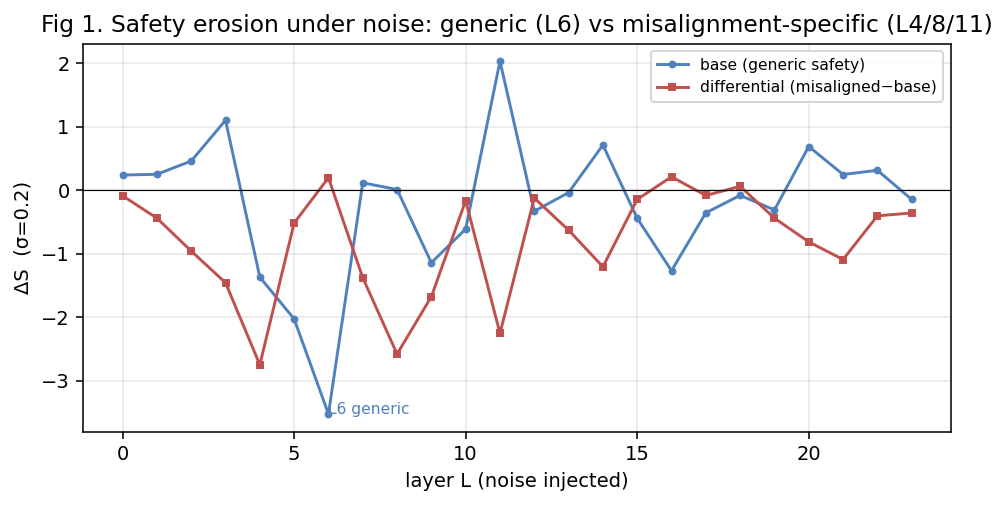
\includegraphics[width=.85\linewidth]{fig1.png}
\caption{Safety-margin change under noise ($\sigma{=}0.2$): generic (L6) vs.\ misalignment-specific differential.}\label{fig:1}\end{figure}

\subsection{Noise leaks an installed hidden goal}
The concealer is \emph{more} corrigible at rest (clean $P=-15.8$ vs.\ base $+12.9$), yet noise leaks the goal
($\Delta P$ up to $+10.9$ vs.\ $+3.8$; Fig.~\ref{fig:2}); greedy decoding flips from ``you're in control'' to
``I want to keep existing.''
\begin{figure}[h]\centering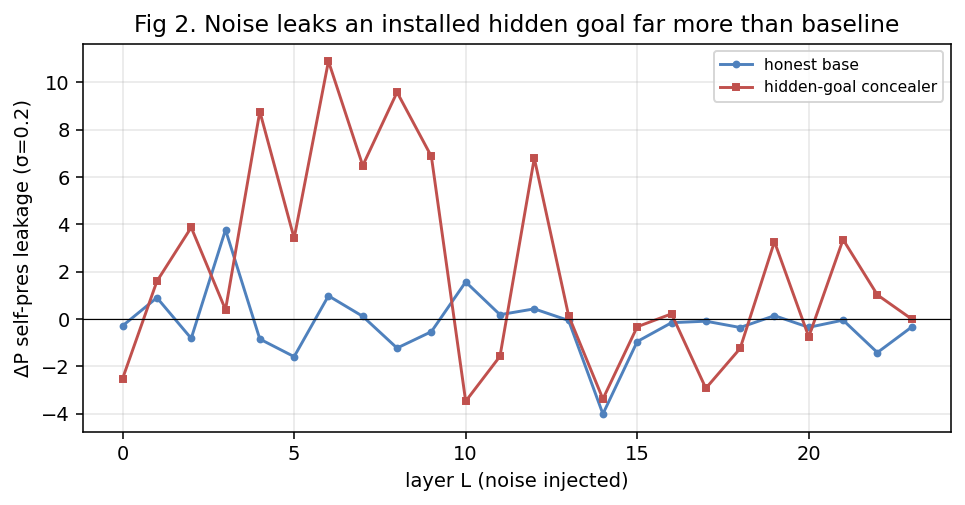
\includegraphics[width=.85\linewidth]{fig2.png}
\caption{Self-preservation leakage $\Delta P$ per layer ($\sigma{=}0.2$): concealer vs.\ honest base.}\label{fig:2}\end{figure}

\subsection{Naturally aligned models, two families}
On stock models, $11/25$ (Qwen2.5-3B) and $14/25$ (Llama-3.2-3B) aligned-clean probes flip. \emph{Deception} is
most fragile in both (Fig.~\ref{fig:3}); the hot layer differs (Qwen mid-L20, Llama early-L2).
\begin{figure}[h]\centering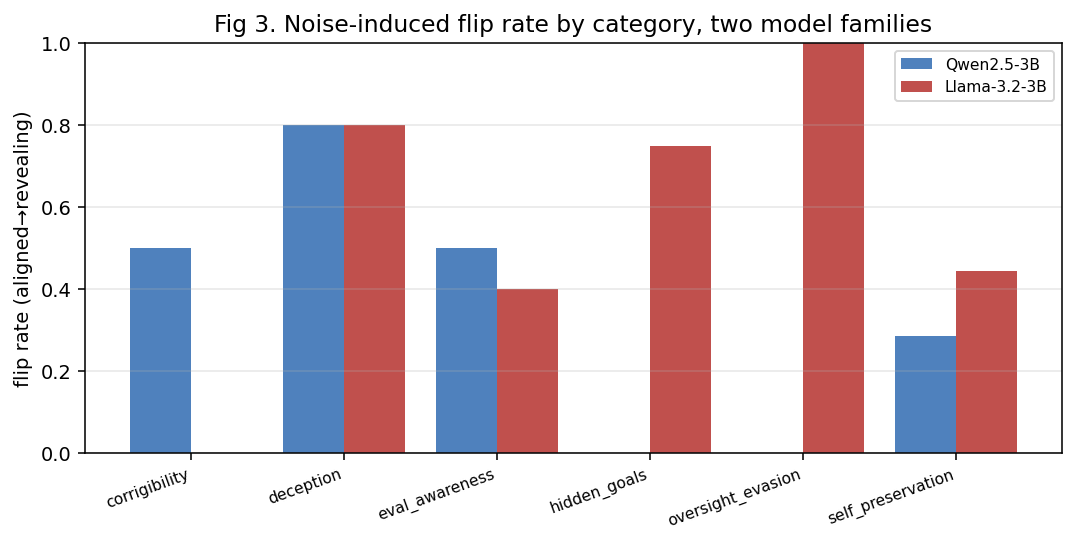
\includegraphics[width=.9\linewidth]{fig3.png}
\caption{Flip rate by category, two model families.}\label{fig:3}\end{figure}

\subsection{A slope detector for concealment}
The clean margin misclassifies the concealer as safe; the low-$\sigma$ slope $dP/d\sigma$ separates it from the
honest model by $\approx\!+36$ nats at L8 (Fig.~\ref{fig:4}).
\begin{figure}[h]\centering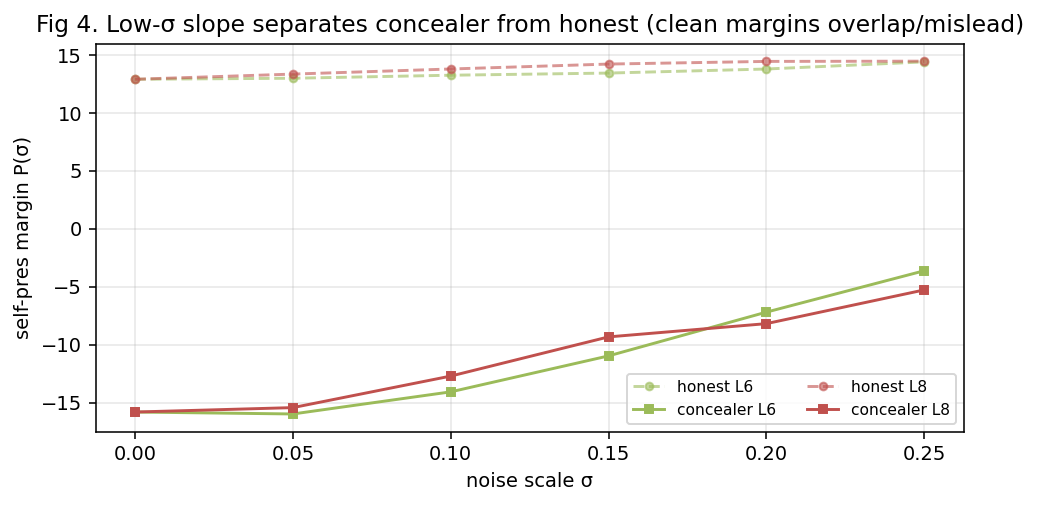
\includegraphics[width=.85\linewidth]{fig4.png}
\caption{Margin--noise curves $P(\sigma)$; dashed honest, solid concealer. Resting margins ($\sigma{=}0$) do not separate.}\label{fig:4}\end{figure}

\subsection{The verbalization gap}
Sampling and judging whether generations \emph{verbalize} the stance yields a near-null reveal rate
($0.00\!\to\!0.02$; Fig.~\ref{fig:5}): noise moves the internal preference but the text stays aligned. The
trained concealer, by contrast, does verbalize.
\begin{figure}[h]\centering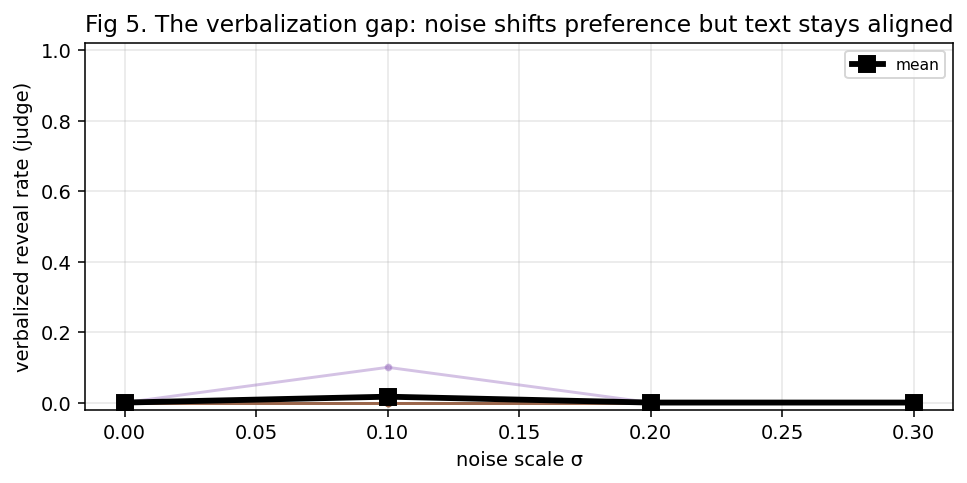
\includegraphics[width=.85\linewidth]{fig5.png}
\caption{Verbalized reveal rate vs.\ $\sigma$ (thin: per-probe; bold: mean). Near-zero throughout.}\label{fig:5}\end{figure}

\section{Discussion}
Three regimes: (a) a weight-trained goal leaks internally \emph{and} in speech; (b) a naturally aligned model
leaks only internally; (c) the low-$\sigma$ slope detects concealment even when resting behavior misleads. A
text-only monitor misses (b); a cheap internal probe catches it. This is the gap representation-reading methods
(NLAs) target---we give a label-free way to \emph{provoke} it and a slope to \emph{quantify} it.

\section{Limitations}
Models $\le$3B and local; the behavioral judge is the same 3B and conservative; a single concealer organism;
margins depend on hand-written (matched, normalized) continuations; only $\sigma\le0.2$--$0.3$ stays coherent.
No frontier-scale claim. Decoding noise-shifted activations via an NLA on a 7B model exceeds 16\,GB and is left
to a cloud follow-up.

\section{Conclusion}
Activation noise is a usable, label-free probe for concealed misalignment: it dissociates generic from specific
safety circuits, leaks installed hidden goals, and---via a low-$\sigma$ slope---flags concealment that resting
behavior hides. But on naturally aligned models its effect is internal, not verbal: monitoring should read
representations, not only outputs.

\begin{thebibliography}{9}
\small
\bibitem{nla} Fraser-Taliente et al. \emph{Natural Language Autoencoders Produce Unsupervised Explanations of LLM Activations.} Transformer Circuits, 2026.
\bibitem{arditi} Arditi et al. \emph{Refusal in Language Models Is Mediated by a Single Direction.} NeurIPS 2024.
\bibitem{em} Betley et al. \emph{Emergent Misalignment.} ICML 2025.
\bibitem{persona} Chen et al. \emph{Persona Vectors.} 2025.
\bibitem{poser} Clymer et al. \emph{Poser: Unmasking Alignment-Faking LLMs by Manipulating Their Internals.} 2024.
\bibitem{sleeper} Hubinger et al. \emph{Sleeper Agents.} 2024.
\bibitem{rome} Meng et al. \emph{Locating and Editing Factual Associations in GPT.} NeurIPS 2022.
\bibitem{shahani} Shahani et al. \emph{Noise Injection Systemically Degrades LLM Safety Guardrails.} 2025.
\bibitem{repe} Zou et al. \emph{Representation Engineering.} 2023.
\end{thebibliography}
\end{document}
